\title{\vspace{160px} \textbf{\huge{Telecommunication Theory}} \\\vspace{17.5px} \LARGE{Lab report 4}  \vspace{10px}}
\author{Alessandro Trigolo}
\date{December 4, 2023}

\begin{document}
\maketitle \newpage

\section*{Objective}
The laboratory's goal is to implement and analyze the effectiveness of the optimal correlator receiver implemented in the three modulation techniques, already explained during laboratory work 3. This kind of receiver uses the \textbf{maximum likelyhood} approach and the \textbf{correlation integral} to detect properly the symbol. The idea behind this operation is rather simple: the correlation integral takes a known input sample signal, like the signal of the 1-symbol, and shifts it along all the received - and disturbed - signals. When the shifted sample lines up with a part of the disturbed signal, this interval is very likely to represent the same symbol as the sample and the symbol detection will be performed successfully.

\section*{Source code and plots}
\lstset{style = MATLAB}
The source code provided in this section has to be appended to the code produced during laboratory 3 so there won't be any explanations regarding the above-mentioned code. Alongside the lines of code, there will be some explanatory comments to make the lab 4 source code more readable.

\subsection*{Task 1}
The first task of the lab work asked to add to the already-written code the MATLAB script for the optimal correlation receiver. Of course, the receiver has to be implemented in the three modulation techniques. In all three techniques, the optimal receiver is coded inside in a \textsl{for loop} that cycles through all the symbols, so from 1 to $N$.

\subsubsection*{BASK}
The first optimal correlator receiver to implement is for the BASK modulation. After creating the integrator vector, inside the for loop, the correlator multiplication is achieved by multiplying element-wise the carrier signal and the disturbed BASK signal. After that, with the help of the cumulative sum (\texttt{cumsum}) function the integral is discretely calculated. At the end of the for loop, the detection is achieved by comparing the symbols in the integrator signal with half of the carrier energy, which is the threshold for the BASK-modulated signal.

\begin{lstlisting}
% preparation for integrator output signal 
integrator = []; 

for k = 1 : N
    % indexes of the signal segment
    index = (1:200) + (k-1)*200;

    % correlator multiplication 
    sM1 = s0 .* BASK_with_noise(index);  

    % calculate continuous integral using a finite sum
    integrator = [integrator, cumsum(sM1)]; 

    % symbol detection is achieved by comparing the integrator signal with half of the carrier energy
    detected_symbols(k) = integrator(end) > Eb/2;
end
\end{lstlisting}

\subsubsection*{BFSK}
In the BFSK modulation technique, there are two carriers instead of one. This means that there will be two signal integrators that have to be produced inside the for loop. After generating the integrator indexes, it is necessary to create the correlator multiplication for the first and the second integrators. To create the actual integrators, as we did in the BASK technique, the \texttt{cumsum} function will be utilized to make the discrete sum. At the end of the for loop, to detect the symbols, a check has to be done between the first and the second integrator which respectively represents the 1 symbol carrier and the 0 symbol carrier. 

\begin{lstlisting}
% preparation for two integrator output signals
integrator1 = []; 
integrator2 = [];

for k = 1:N
    % indexes of the signal segment
    index = (1:200) + (k-1)*200;

    % 1st correlator multiplication 
    sM1 = s1 .* BFSK_with_noise(index);  

    % calculate 1st continuous integral using a finite sum
    integrator1 = [integrator1, cumsum(sM1)];


    % 2nd correlator multiplication 
    sM2 = s2 .* BFSK_with_noise(index);

    % calculate 2nd continuous integral using a finite sum
    integrator2 = [integrator2, cumsum(sM2)];

    % detects symbols
    detected_symbols(k) = integrator1(end) > integrator2(end);
end
\end{lstlisting}

\subsubsection*{BPSK}
The third optimal correlator receiver to implement is the one for the BPSK technique. In this case, the script is very similar to the one produced for the BASK technique. The only line of code that changes is the detection algorithm: in this case, the threshold is zero. The important thing to notice is that if the integrator signal is lower than zero this means that the symbol one is detected because to generate the BPSK the input signal has to be converted in a \textsl{NRZ} (Non-Return-to-Zero) signal. This means that, after the conversion, the negative voltage identifies the symbol one.

\begin{lstlisting}
% preparation for integrator output signal 
integrator = [];    

for k = 1 : N
    % indexes of the signal segment
    index = (1:200) + (k-1)*200;

    % correlator multiplication 
    sM1 = s0 .* BPSK_with_noise(index);  

    % calculate continuous integral using a finite sum
    integrator = [integrator, cumsum(sM1)]; 

    % symbol detection is achieved by comparing the integrator signal with the 0-threshold
    detected_symbols(k) = integrator(end) < 0;
end
\end{lstlisting}

\subsection*{Task 2}
The second task demanded plotting on one image the disturbed signal and the optimal correlation receiver signal: the \texttt{subplot} function was utilized. The script is very similar to the three modulation techniques, so it is shown only the script used for the BFSK modulation, which is the more complex one.

\begin{lstlisting}
subplot(311), plot(BFSK_intervals, BFSK_with_noise), grid on; % plot disturbed signal
xlabel('Time [s]'), ylabel('BFSK signal with noise'); % labels
ylim([-4 4]); % limits

subplot(312), plot(BFSK_intervals, integrator1), grid on; % plot 1st integrator
xlabel('Time [s]'), ylabel('1st Correlator output'); % labels
ylim([-50, 150]); % limits


subplot(313), plot(BFSK_intervals, integrator2), grid on; % plot 2nd integrator
xlabel('Time [s]'), ylabel('2nd Correlator output'); % labels
ylim([-50, 150]); % limits
\end{lstlisting}

\noindent As a reference, the transmitted symbols in all three modulation types are the same: \texttt{[ 0 0 1 0 1 0 0 0 1 1 1 1 0 1 1]}. The symbols are plotted in the following figure.

\begin{figure}[h!]
    \centering
    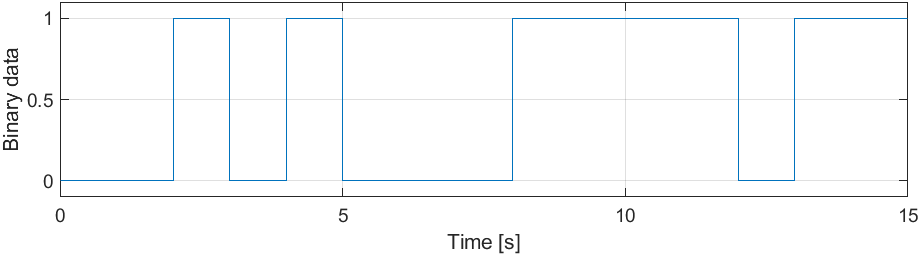
\includegraphics[width = .7\textwidth]{lab-4/imgs/initial-data.png}
\end{figure}

\FloatBarrier\noindent After running the script, for the BASK modulation technique the two plotted signals are presented in the following figure. Noticeably, when the integrator signal exceeds the red threshold the symbol one is detected.

\begin{figure}[h!]
    \centering
    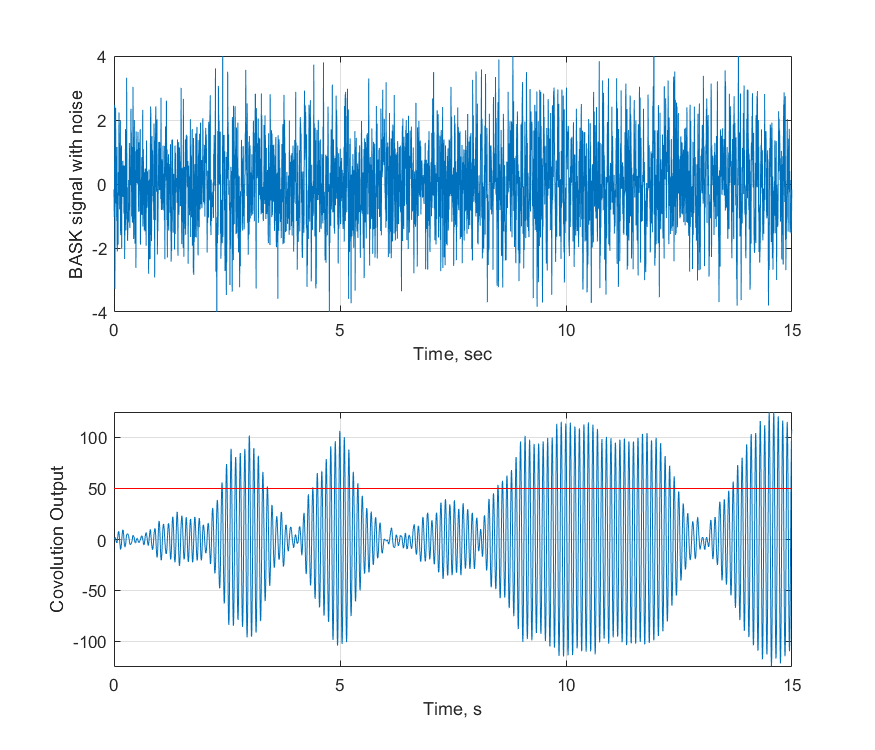
\includegraphics[width = .7\textwidth]{lab-4/imgs/BASK.png}
\end{figure}

\FloatBarrier\noindent In the BFSK modulation technique the integrator plots are reasonably two instead of one: the first represents the carrier for the 1 symbol while the second one refers to the 0 symbol. Notably, when the first carrier is greater than the second the 1 symbol is detected.
\begin{figure}[h!]
    \centering
    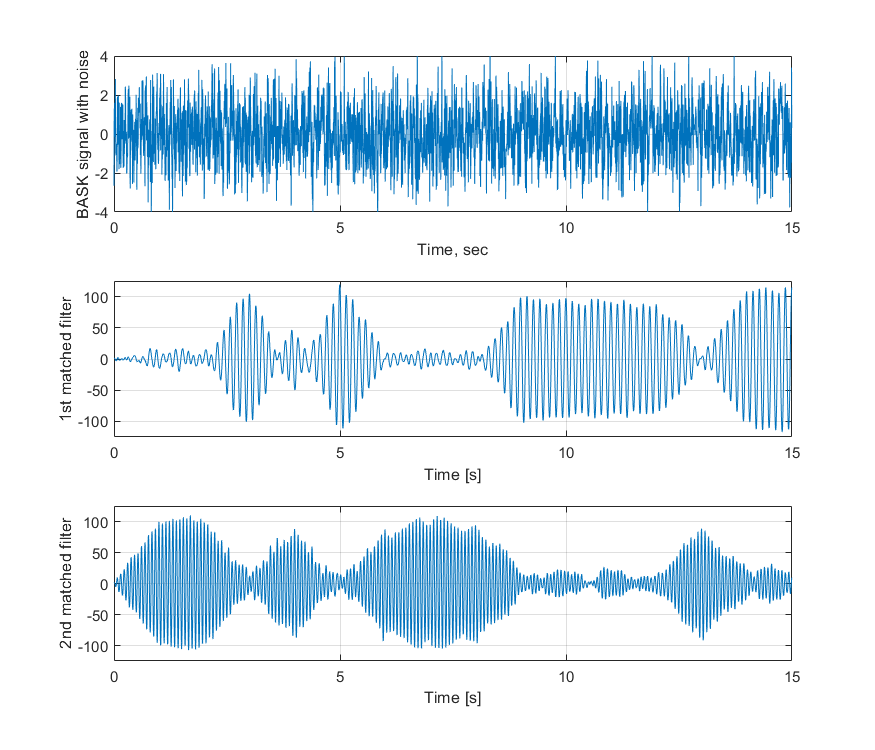
\includegraphics[width = .7\textwidth]{lab-4/imgs/BFSK.png}
\end{figure}

\FloatBarrier\noindent On the other hand, in the last modulation - the BPSK - a 1-symbol is detected when the integrator signal is lower than the threshold, which is zero. The following figure shows this process.

\begin{figure}[h!]
    \centering
    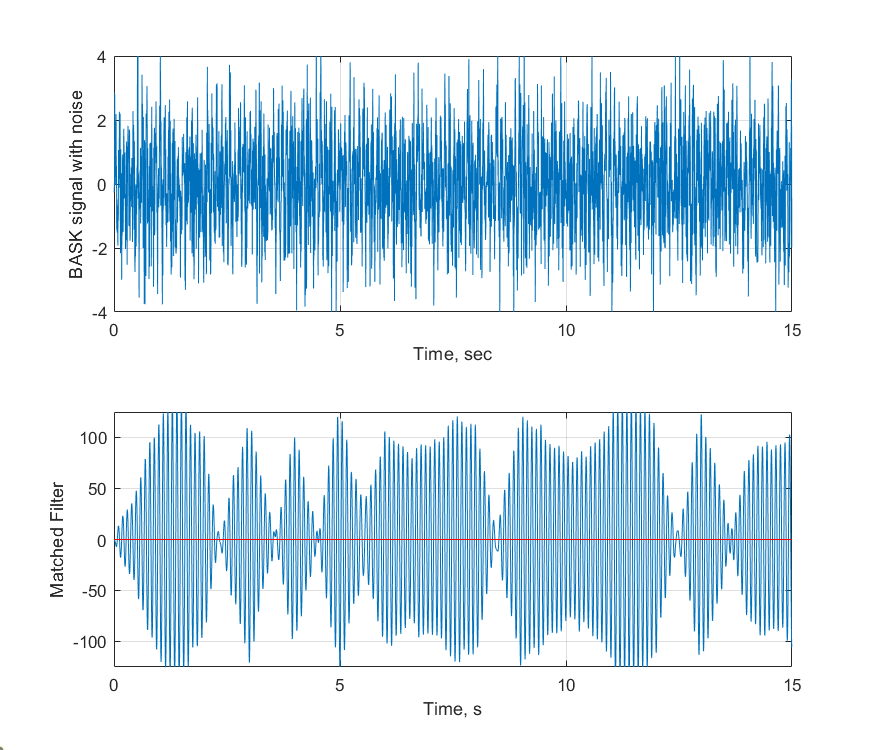
\includegraphics[width = .7\textwidth]{lab-4/imgs/BPSK.png}
\end{figure}


\FloatBarrier

\subsection*{Task 3}
A comparison between the initial data and the detected data has to be performed. A very simple script is needed to achieve such a comparison: the detected data will be compared with the initial binary sequence element-wise and then the BER value will be calculated. For clarity, in the end, the SNR value is displayed along with the total number of transmitted symbols $N$, the number of errors that occurred during the transmission and, of course, the BER value.

\begin{lstlisting}
check = binary_sequence == detected_symbols; % check element-wise
errors = N - sum(check); % counts errors
BER = errors / N; % calculates Bit Error Rate

disp('SNR:              ' + SNR);
disp('Total symbols:    ' + N);
disp('Errors:           ' + errors);
disp('BER:              ' + BER);
\end{lstlisting}

\noindent To analyze the impact of the SNR value during the transmission, a set of 10000 symbols will be transmitted with different SNR values. The results obtained are summed up in the following table.

\begin{table*}[h!]
    \centering
    \renewcommand{\arraystretch}{1.5}
    \begin{tabular}{|c|c c c|}
        \hline
        \multirow{2}{*}{\textbf{SNR} value} &  \multicolumn{3}{c|}{\textbf{BER} value} \\
        & \textsl{BASK} & \textsl{BFSK} & \textsl{BPSK} \\\hline\hline
        20 & 0 & 0 & 0 \\
        15 & 0 & 0 & 0 \\
        10 & 0.0128 & 0.0008 & 0 \\
        7 & 0.0582 & 0.0151 & 0.0009 \\
        5 & 0.1021 & 0.037 & 0.0062 \\
        2 & 0.1894 & 0.1019 & 0.0376 \\
        0 & 0.246 & 0.156 & 0.0772 \\\hline

    \end{tabular}
    \renewcommand{\arraystretch}{1}
\end{table*}

\FloatBarrier\section*{Conclusions}
Noticeably, by analyzing the table that contains the BER values associated with the SNR values we can see a drastic increase in the error rate as the signal gets weaker, specifically in the BASK and BFSK modulations. The table also shows that the BPSK modulation technique is more effective and reliable in noisy environments than the other two modulations: when the SNR value is 7 - meaning that the signal is almost 5 times stronger than the noise - the BPSK BER value is very low (9 errors out of 10000) while in the BASK modulation, it is more than 50 times higher (528 errors in 10000 transmitted symbols).



\end{document}